\documentclass[12pt]{article}
%Gummi|065|=)
\usepackage{amsmath, amsfonts, amssymb}
\usepackage[margin=0.5in]{geometry}
\usepackage{xcolor}
\usepackage{graphicx}

\newcommand{\off}[1]{}
\DeclareMathSizes{20}{30}{20}{18}

\newcommand{\two }{\sqrt[3]{2}}
\newcommand{\four}{\sqrt[3]{4}}
\newcommand{\red}{\begin{tikz}[scale=0.25]
\draw[fill=red, color=red] (0,0)--(1,0)--(1,1)--(0,1)--cycle;\end{tikz}}
\newcommand{\blue}{\begin{tikz}[scale=0.25]
\draw[fill=blue, color=blue] (0,0)--(1,0)--(1,1)--(0,1)--cycle;\end{tikz}}
\newcommand{\green}{\begin{tikz}[scale=0.25]
\draw[fill=green, color=green] (0,0)--(1,0)--(1,1)--(0,1)--cycle;\end{tikz}}

\usepackage{tikz}

\title{Aspects of Ratner Theory}
\author{John D Mangual}
\date{}
\begin{document}

\fontfamily{qag}\selectfont \fontsize{12.5}{15}\selectfont

\maketitle

\noindent In this note we look at quantitative Ratner theory\dots the typical paradox in academica:
\begin{itemize}
\item there are techniques and results known to a few experts
\item subject hardly known outside of that clique (even among other academics)
\end{itemize} 
If you are Elon Lindenstraus or Grigory Margulis or whoever, yeah\dots you know what's going on.  \\ \\
Logically these problems are difficult because they say obvious things about common household objects. Why would you expend so much effort to prove something that's clearly true? \\ \\
Nobody told me to work on this.  Suddently I am taking on considerations like these. Here's one way into Ratner Theory.  {Legendre} proved in 1798 that:
\begin{center}
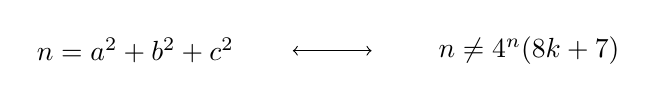
\begin{tikzpicture}  
\node at (0,0){$n = a^2 + b^2 + c^2$};
\draw[<->](2,0)--(3,0);
\node at (5,0){$n \neq 4^n(8k+7)$};
\end{tikzpicture}
\end{center}
Such a pleasant theorem.  It's quite natural to draw these thing solutions on a sphere, and all kinds of beautiful patterns emerge.  \\
\includegraphics[width=3in]{ratner-01.png}\hfill
\includegraphics[width=3in]{ratner-02.png}\\
The most natural conclusion would be these colored dots are getting evenly spread out over the ball (or sphere).  And we say the solutions to the sum of three squares problem are getting  \textit{equidistributed} as $n \to \infty$.  \\ \\
This turns out to be a very very difficult problem, only solved in 1987 by William Duke and the solution itself we very difficult to decode buried in the middle of other results.  \\ \\
Even finding one solution (instead of proving that solutions evenly spread out) is about 20 or 30 pages of algebra, that can't get shortened.

\newpage

\noindent So I think one way in this mess is to try to ask a very simple question and to try to demand a simple answer.  Let's back down a little bit:
$$ n = a^2 + b^2 + c^2 + d^2 $$
\textbf{Every positive integer is the sum of four perfect squares.} This was prove a long time ago by Lagrange.  \\ \\
These are ``solved" in the sends that a community of experts considers them solved.  Yet, I consider them open because nobody outside of that group can look inside and agree with their conclusion. \\ \\
A few more toy examples.  Here's one by Fermat about \textbf{primes as the sum of two squares}:
$$ p = a^2 + b^2 \text{ if and only if } p = 4k+1 $$
and we can ask about the angle $\theta = \tan^{-1}(\frac{b}{a})$ of the vector $(a,b) \in \mathbb{Z}^2$, and it is also evenly distribution as $p \to \infty$. If you're an expert these are pretty clear.  As a beginner, amateur, outsider whatever, these examples start to look pretty weird. \\ \\
These are my buy-ins to Ratner Theory.  The problems you look at every day, and here we put a microscope.\footnote{There should be many problems of this kind, with a basic phrasing, and a far-reaching answer.  Gradually, we'll add to this list.}
\vfill



\begin{thebibliography}{} 

\item \dots 

\end{thebibliography}



\end{document}